\section{The reconstruction ladder}\label{sec:ladder}

We separate the \emph{primitive} from \emph{supplied ingredients} and index
rungs by the minimal ingredient each requires.

The primitive is:
\begin{itemize}
\item \textbf{Causal / accessibility order.} A strict partial order on
  events (in the continuum models, Minkowski causal precedence;
  null-inclusive).
\end{itemize}

The supplied ingredient symbols (these form branches, not one linear
hierarchy) are:
\begin{itemize}
\item \textbf{M---global event-density calibration.} The conversion between
  event count and physical volume in the declared sampling model.
\item \textbf{O---observer chain with clock labels.} A timelike chain
  carrying ordered tick labels (an operational clock), defining a radar
  protocol.
\item \textbf{R---oriented synchronized reference.} A second beacon chain
  with calibrated separation, fixing a spatial side.
\item \textbf{A---observer atlas.} Multiple overlapping observer charts.
\item \textbf{W---local measure profile / weights.} The physical volume
  element relative to the support sampling measure, normalized to unit mean
  over the declared support, so that all scale information belongs to M and
  W carries only position dependence; a constant profile is therefore
  $\mathrm{W} = 1$ and supplies nothing beyond M.
\end{itemize}

\Tref{tab:rungs} lists the rungs (minimal ingredient $\to$ what is
reconstructed).

\begin{table}[t]
\caption{Rungs of the reconstruction ladder: the minimal ingredient set,
what it reconstructs, and what bounds it.}
\label{tab:rungs}
\begin{tabularx}{\textwidth}{@{}llXX@{}}
\toprule
Rung & Ingredient & Reconstructed & Bounded by \\
\midrule
\multicolumn{4}{@{}l}{\emph{Measure branch: order, ${+}$\,global density, ${+}$\,local measure}} \\
R0 & order only & flat-sprinkling dimension estimate; uncalibrated chain
  statistics & manifold/model assumptions; no metric scale \\
R1 & order + M & timelike proper time (interval cardinality $\to$ volume
  $\to$ $\tau$) & needs a density \\
R5 & order + M + W & volume under conformal ambiguity; coarse-graining
  stability & global and local measure supplied \\
\midrule
\multicolumn{4}{@{}l}{\emph{Observer branch: order, ${+}$\,clocked chain, ${+}$\,orientation, ${+}$\,charts}} \\
R2 & order + O & radar time; unsigned radar distance & sign undetermined \\
R3 & order + O + R & signed coordinates; Lorentz map between protocols &
  supplied orientation \\
R4 & order + O + R + A & atlas transition maps (Poincar\'e); invariant
  agreement & oriented, calibrated charts \\
\bottomrule
\end{tabularx}
\end{table}

The two branches are not of the same kind, and \tref{tab:rungs} groups
them rather than presenting six co-equal rungs. The measure branch---order,
plus a global density, plus a local measure---is the operational form of
the causal-order rigidity theorems plus a volume
element~\cite{malament1977,hkm1976}; it is where the first negative result
bites and where the whole of \sref{sec:capstone} operates. The observer
branch is protocol arithmetic: once a timelike chain with ordered tick
labels, an oriented calibrated beacon and overlapping charts have been
supplied, a coordinate system's worth of structure has been supplied, and
radar coordinates follow close to definitionally---those rungs validate
bookkeeping, and their bounding result, the reflection degeneracy, is the
protocol's own symmetry made explicit rather than a discovered obstruction.
The ledger's value is the explicit per-rung accounting; the theorem content
lives on the measure branch.

Three negative results bound the ladder from below (\sref{sec:negative}):
conformal scale is not fixed by order alone (motivating M and W); a single
observer gives only unsigned distance (motivating R); and finite signal
speed alone does not give Lorentzian structure. \Fref{fig:ladder}
summarizes the ladder.

\begin{figure}[t]
\centering
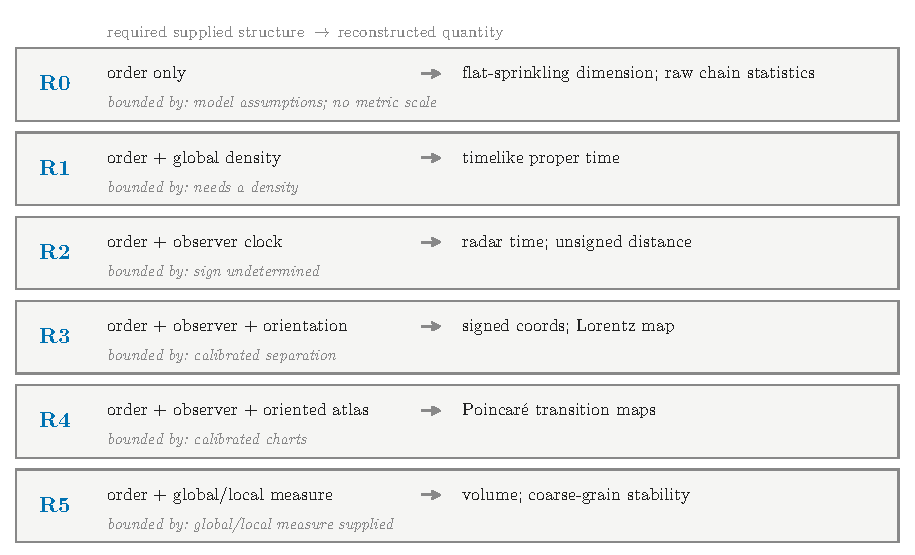
\includegraphics[width=0.95\textwidth]{figures/fig1_ladder.pdf}
\caption{The reconstruction dependency ledger. Each row names a minimal
ingredient set and the quantity it unlocks; the observer and measure rows
are branches rather than one cumulative linear chain. The ``bounded by''
line records what that ingredient set still does not supply.}
\label{fig:ladder}
\end{figure}
